%!TEX TS-program = xelatex
\documentclass[]{shiltemann-cv}
\addbibresource{publications.bib}

\begin{document}
\header{Saskia}{Hiltemann}
       {Doctoral Researcher, Bioinformatics \& Training}


% In the aside, each new line forces a line break
\begin{aside}
  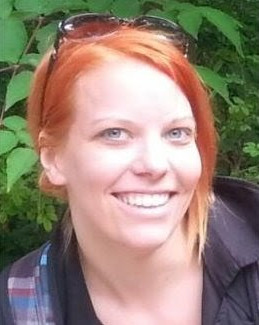
\includegraphics[width=75pt]{foto.jpg}
  \section{About}
    Laakkade 378
    2521 XV, Den Haag
    The Netherlands
    ~
    zazkia@gmail.com \faEnvelope
    shiltemann \faGithub \ \faTwitter \ \faLinkedin
    \
  \section{Languages}
    Bilingual Dutch/English
    German \& French
  \section{Skills}
    Python, C, C++, Galaxy, Docker, Jekyll
\end{aside}

\section{Interests}

Bioinformatics, Training, Community Building, Genome Sequencing, Data Anlysis, Workflows, Automation, Visualisation, Best Practices, Cancer Research, Microbiome Analysis, Infosec, CTF, Traveling, Hiking, Reading, Puzzles.

\section{Education}

\begin{entrylist}
  \entry
    {Since 2012}
    {Ph.D. {\normalfont candidate in Bioinformatics}}
    {Erasmus Medical Center}
    {\emph{Bioinformatics for Everybody.}}
  \entry
    {2008–2010}
    {M.Sc.}
    {LIACS, University of Leiden \& TU Delft}
    {Computer Science\\
    Specialization in Bioinformatics}
  \entry
    {2005–2008}
    {B.Sc.}
    {LIACS, University of Leiden}
    {Computer Science}
  \entry
    {2002–2005}
    {B.Sc. course work}
    {University of Leiden}
    {Physics \& Astronomy}
  \entry
    {2002}
    {High School (VWO)}
    {Alfrink College, Zoetermeer}
    {Specialization in Science \& Technology}
\end{entrylist}

\section{Work Experience}

\begin{entrylist}
 \entry
    {Current}
    {Erasmus Medical Center, Rotterdam}
    {}
    {Bioinformatician and Doctoral Researcher
     \begin{itemize}
     \item \emph{Software Development and Pipeline building}
     \item \emph{Training Development and Delivery}
     \item \emph{Galaxy System's Administrator}
     \item \emph{Microbiota Analysis and Antibiotic Resistance Detection}
     \item \emph{Prostate Cancer Analysis}
     \end{itemize}}
  \entry
    {2010-2012}
    {After's Cool, The Hague}
    {Tutor of High School Students.}
    {Tutor of High School Students. \emph{Math, Physics, Chemistry}}
  \entry
    {2002-2010}
    {Self-Employed}
    {}
    {Tutor of High School Students. \emph{Math, Physics, Chemistry}}
\end{entrylist}

\section{Projects}

\begin{entrylist}
  \entry
    {2018}
    {Clinical Microbiota Analysis Pipeline}
    {ErasmusMC}
    {Development of an analysis pipeline for use in daily clinical diagnostics of sepsis patients for Streeklab Haarlem.}
  \entry
    {2016-18}
    {Galaxy Training Materials}
    {GalaxyProject}
    {Co-developed infrastructure for the collaborative development of Galaxy training materials, as well as development of several training manuals on topic of Metagenomics, Galaxy Development and Visualisation}
\end{entrylist}

\newpage
\newgeometry{left=3cm}

\begin{entrylist}
  \entry
    {2016}
    {Galaxy CTF}
    {Galaxy Community Conference 2016}
    {Together with Helena Rasche, built a framework and 28 challenges for a “Capture the Flag” event based on Galaxy. Tasks included exploiting recently patched security bugs within Galaxy, Docker security issues, exploring new Galaxy features, and exploiting common bugs in Galaxy tools. Approximately 16 people participated in the competition. The infrastructure for the competition was released afterwards to allow others to re-use it for educational purposes.}
   \entry
     {2016-18}
     {Galaxy Interactive Environment Development}
     {GalaxyProject}
     {Created Galaxy Interactive Environments (GIEs) for several applications, including Phinch for metagenomic data visualisation and Ethercalc.}
   \entry
    {2012-18}
    {Galaxy Tool Development}
    {GalaxyProject}
    {I have integrated over 100 tools into the Galaxy Tool shed, including Complete Genomics Tools, Mothur for 16S rRNA sequence Analysis, Circos for visualisation, and more. Member of Galaxy's IUC team of tool developers.}
\end{entrylist}

\section{Publications}

\nocite{*} % Include references even those which weren't cited
\printbibliography[sorting=chronological, title={~}]

\section{Training}

%%% This piece of code has been commented by Karol Kozioł due to biblatex errors.
%
%\begin{refsection}
%  \nocite{*}
%  \printbibliography[sorting=chronological, type=inproceedings, title={international peer-reviewed conferences/proceedings}, notkeyword={france}, heading=subbibliography]
%\end{refsection}
%\begin{refsection}
%  \nocite{*}
%  \printbibliography[sorting=chronological, type=inproceedings, title={local peer-reviewed conferences/proceedings}, keyword={france}, heading=subbibliography]
%\end{refsection}
%\printbibsection{misc}{other publications}
%\printbibsection{report}{research reports}

\end{document}
